\documentclass[12pt]{article}

\usepackage[hidelinks]{hyperref}
\usepackage[margin=0.9in]{geometry}
\usepackage{cite}
\usepackage{etoolbox}
\usepackage{graphicx}
\usepackage{wrapfig}
% \usepackage{savetrees}

% https://tex.stackexchange.com/a/132647
\patchcmd{\thebibliography}{\section*{\refname}}{}{}{}

\begin{document}
\begin{center}
  {\Large An Online Interactive ARIES Visualization}
\end{center}

In CS 186: Intro to Database Systems, students learn about the design and
implementation of relational databases: complex pieces of software that are
responsible for storing and managing data. One of the key challenges in
designing a database is ensuring that data is never lost, even if the database
crashes and later recovers. The de facto standard recovery algorithm---the one
that is taught in nearly every undergraduate course on databases---is called
ARIES, and let me tell you, it's \emph{really} complicated. How complicated?
Well, the original paper that introduced ARIES is a whopping \textbf{69 pages}
long~\cite{mohan1992aries}! In it, the author notes that ``concurrency and
recovery are complex subjects to think about and program for.'' The CS 186
textbook comments on ARIES noting that ``the recovery manager is one of the
hardest components of a DBMS to design and
implement.''~\cite{ramakrishnan2000database}. Due to its complexity, it's rare
to see a professor (or even a textbook) walk through a complete execution of
the algorithm. As a result, students either (a) spend an exorbitant amount of
time struggling to understand ARIES or (b) flat out give up.

\begin{wrapfigure}{r}{0.5\textwidth}
  \centering
  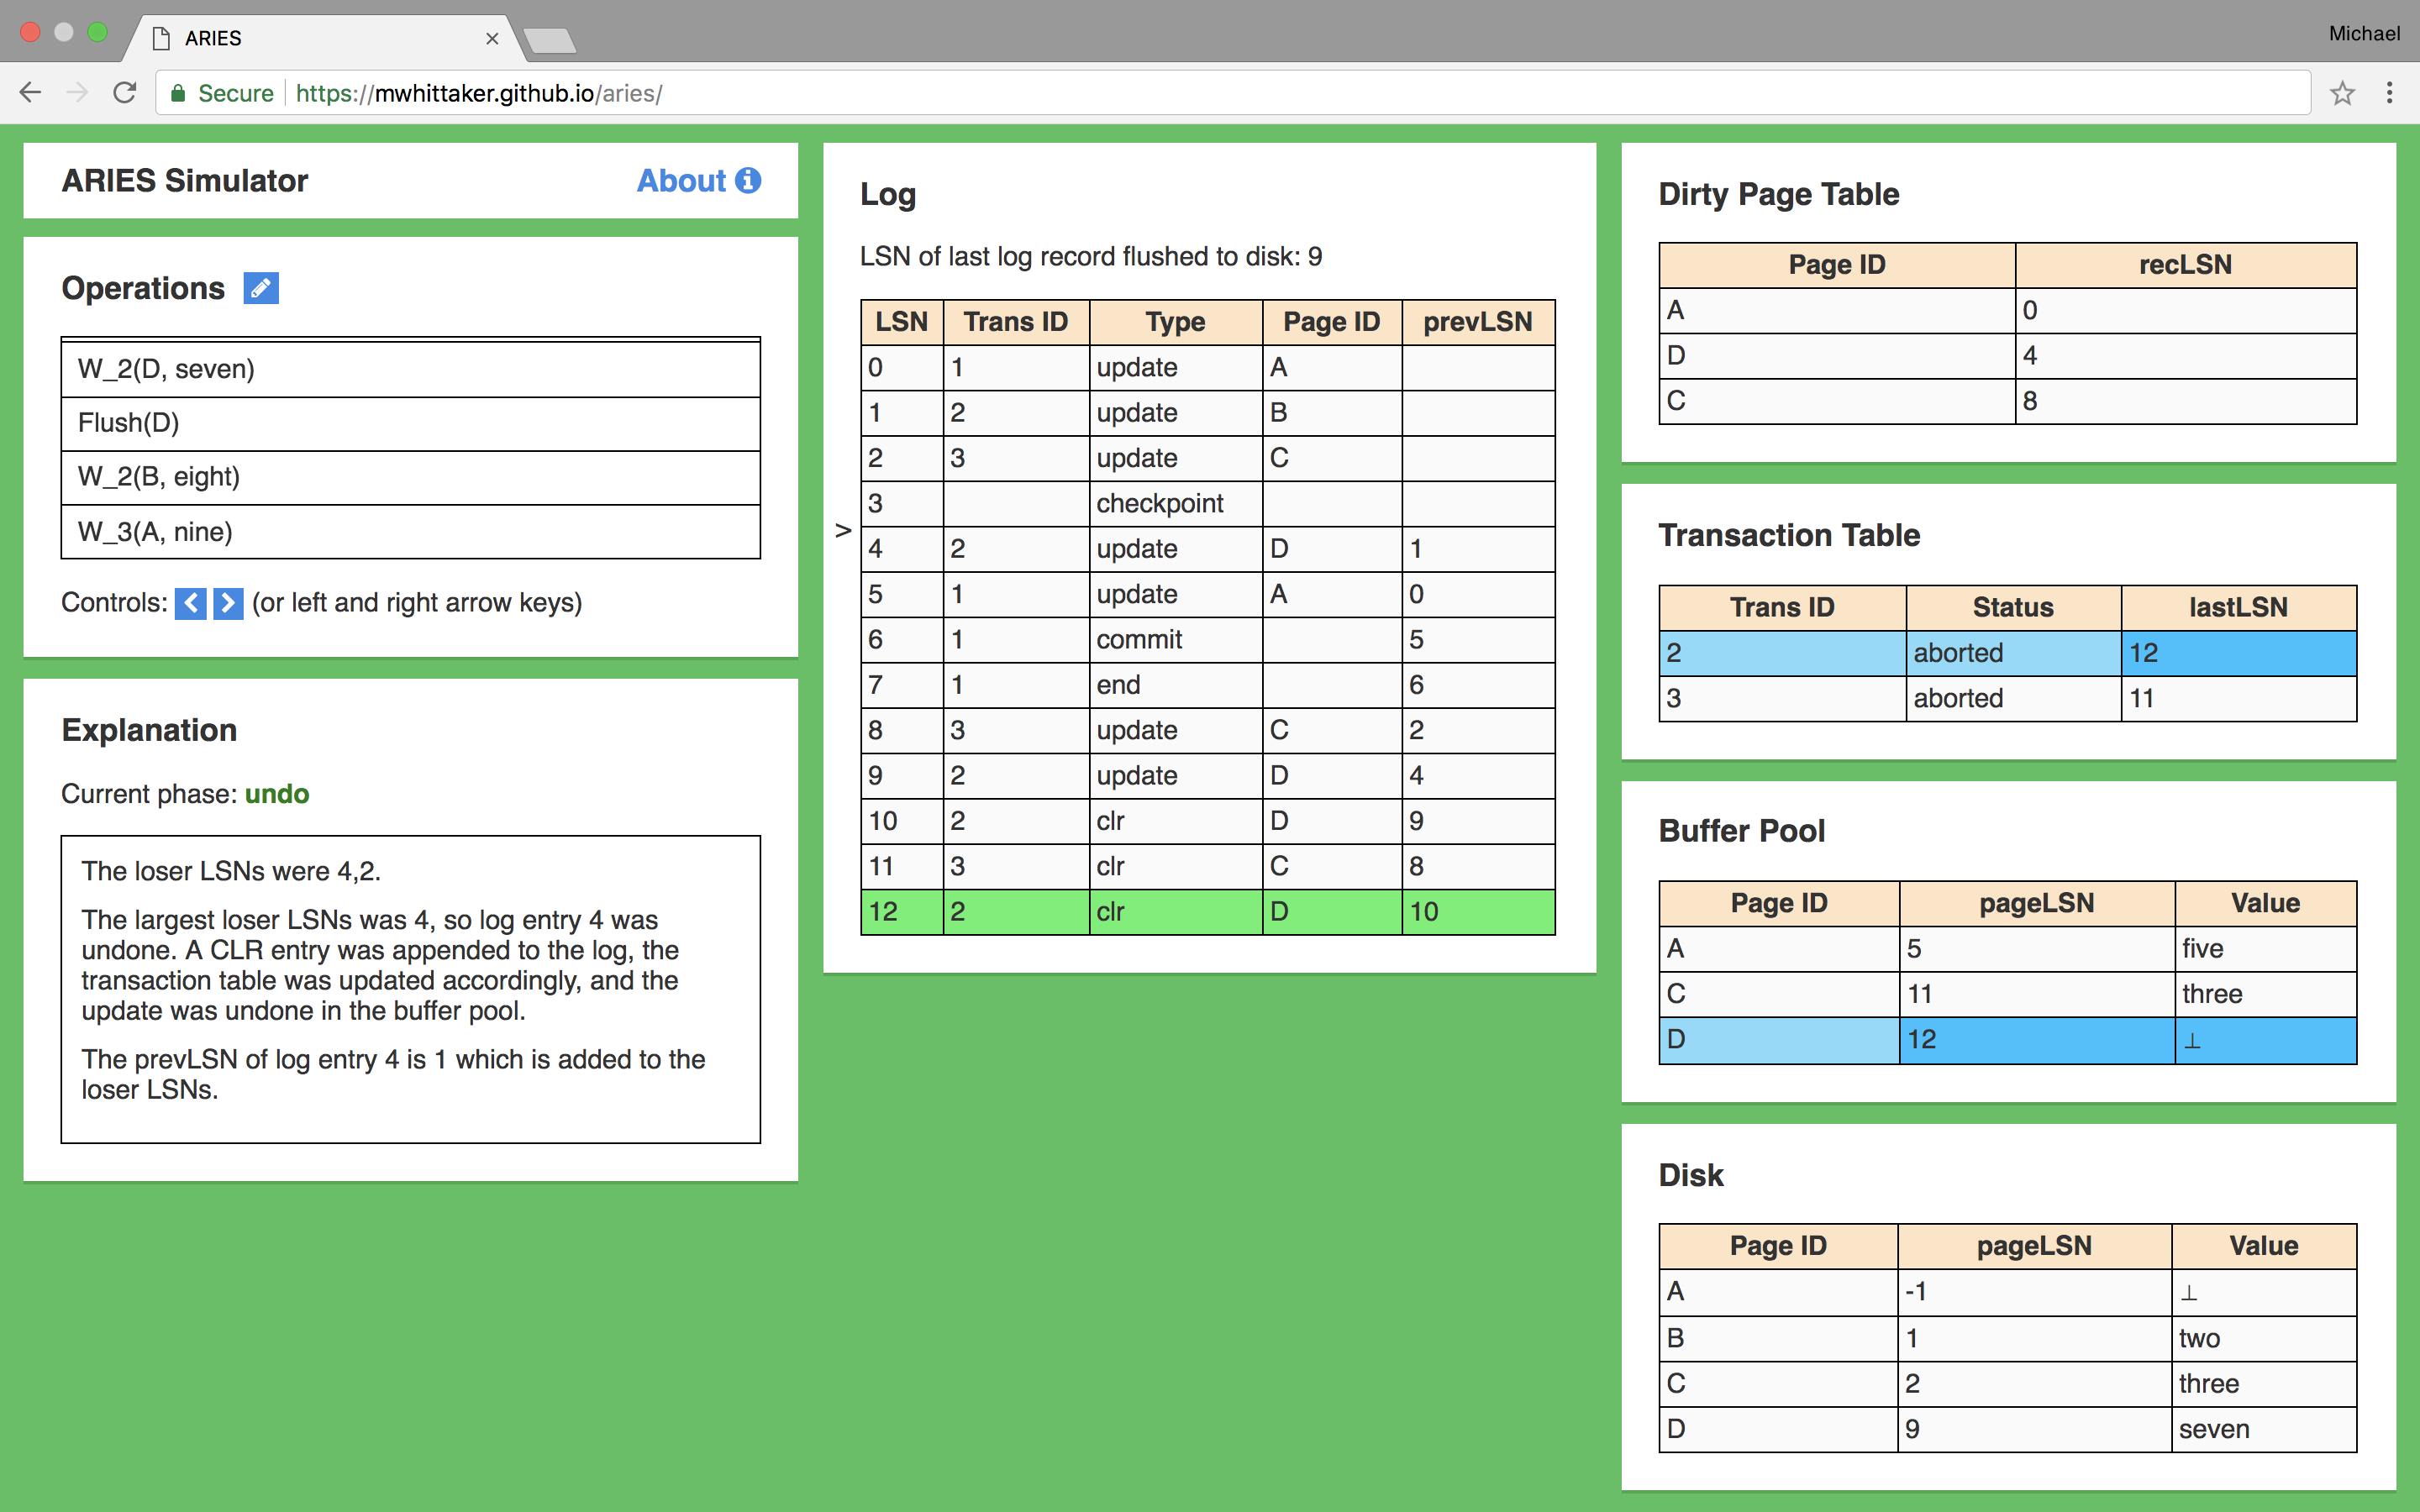
\includegraphics[width=0.5\textwidth]{aries.png}
  \caption{Online ARIES Simulator}\label{LarrysAries}
\end{wrapfigure}

To make it easier for students to understand ARIES, another CS 186 GSI (Larry
Xu) and I jointly implemented an online interactive visualization of ARIES
which is depicted in Figure~\ref{LarrysAries} and can be found online at
\url{https://goo.gl/wxaV4Q}. Students interact with the visualization by
pressing the left and right arrow keys to walk backwards and forwards through
the execution of the algorithm on an arbitrary input. Moreover, the
visualization not only shows \emph{what} ARIES does, it also explains
\emph{why} it does it. The visualization displays auto-generated textual
descriptions of every step of the algorithm so that students can understand why
ARIES works the way it does. Finally, students who want to gain an even deeper
understanding of the implementation details of ARIES can read through the
source code of the visualization which can be found at
\url{https://goo.gl/eBjSMR}.

We deployed the ARIES visualization to the students of CS 186 across two
semesters with great success. In one semester, the visualization amassed 945
page views from 447 unique users. On Piazza, one student commented ``This is a
really really high quality teaching tool IMO. Great job Michael and Larry!
:)''. In Fall 2017, only 19 of the total 1167 Piazza posts were about ARIES
(1.63\%), a remarkably low number for a class of roughly 400 students. The
online visualization has also had impact outside of Berkeley. We have 91 users
from Ithaca, New York suggesting that the visualization is being used at
Cornell University as well. We also have users from 10 different countries
including Canada and the United Kingdom. Overall, the online visualization has
made it significantly easier for students to understand an enormously complex
algorithm, and the visualization has been reused across semesters and across
the globe.

{
  \footnotesize
  \bibliographystyle{plain}
  \bibliography{references}
}
\end{document}
